\documentclass[11pt,a4paper]{article}
\usepackage[catalan]{babel}

% Paquetes necesarios
% preamble.tex

% Codificación y tipografía
\usepackage[utf8]{inputenc}
\usepackage[T1]{fontenc}
\usepackage[catalan]{babel}
\usepackage{lmodern}

% Márgenes y geometría
\usepackage{geometry}
\geometry{left=2.5cm, right=2.5cm, top=2cm, bottom=3cm}
% Estilo de página
\usepackage{fancyhdr}
\setlength{\headheight}{15pt}
\pagestyle{fancy}
\fancyhf{}
\lhead{\textit{Electrònica Física}}
\rhead{\textit{Adrià Rojo}}
\cfoot{\thepage}

% Gráficos y tablas
\usepackage{graphicx}
\usepackage{float}
\usepackage{caption}

% Matemáticas y símbolos
\usepackage{amsmath}
\usepackage{amssymb}

% Hipervínculos
\usepackage{hyperref}

% Espaciado
\usepackage{parskip}  % Quita sangría de párrafos y añade espacio
\usepackage{wrapfig}
\usepackage[backend=biber,style=ieee, autocite=superscript]{biblatex}
\addbibresource{bibliography.bib}

% Fuente y estilo general
\renewcommand{\familydefault}{\rmdefault}

%Definició de la ela geminada per tal que accepti el punt volat del teclat
% \def·#1{%
%   \ifmmode
%     \cdot #1
%     %\csname normal@char\string"\endcsname l%
%   \else%
%     \def\argument{#1}%
%     \if\argument l%
%       \leftllkern=0pt\rightllkern=0pt\raiselldim=0pt%
%       \setbox0\hbox{l}\setbox1\hbox{l\/}\setbox2\hbox{.}%
%       \advance\raiselldim by \the\fontdimen5\the\font
%       \advance\raiselldim by -\ht2%
%       \leftllkern=-.25\wd0%
%       \advance\leftllkern by \wd1%
%       \advance\leftllkern by -\wd0%
%       \rightllkern=-.25\wd0%
%       \advance\rightllkern by -\wd1%
%       \advance\rightllkern by \wd0%
%       \allowhyphens\discretionary{-}{l}%
%       {\hbox{}\kern\leftllkern\raise\raiselldim\hbox{.}%
%         \kern\rightllkern\hbox{l}}\allowhyphens%
%     \else
%       \if\argument L%
%         \leftllkern=0pt\rightllkern=0pt\raiselldim=0pt%
%         \setbox0\hbox{L}\setbox1\hbox{L\/}\setbox2\hbox{.}%
%         \advance\raiselldim by .5\ht0%
%         \advance\raiselldim by -.5\ht2%
%         \leftllkern=-.125\wd0%
%         \advance\leftllkern by \wd1%
%         \advance\leftllkern by -\wd0%
%         \rightllkern=-\wd0%
%         \divide\rightllkern by 6%
%         \advance\rightllkern by -\wd1%
%         \advance\rightllkern by \wd0%
%         \allowhyphens\discretionary{-}{L}%
%         {\hbox{}\kern\leftllkern\raise\raiselldim\hbox{.}%
%            \kern\rightllkern\hbox{L}}\allowhyphens%
%       \else
%         #1
%       \fi
%     \fi
%   \fi
%   }
% Título
\title{\textbf{CMOS: Història, fonaments i funcionament i aplicacions}}
\author{Adrià Rojo}
\date{\today}

\begin{document}

\maketitle
\thispagestyle{empty}
% Resumen
\begin{abstract}
    BLABLA
\end{abstract}

\section{Introducció}
% Introducir brevemente qué es CMOS, su importancia en la electrónica digital y qué estructura tendrá el trabajo.

Un semiconductor-òxid-metall complementari (\textit{Complementary-Metal-Oxide Semiconductor}) o CMOS, és un tipus de tecnologia que combina un parell simètric de nMOS i pMOS connectats de forma complementària per poder fer operacions lògiques de forma eficient\autocite{wiki:CMOS}. 

Aquesta tecnologia és la base d'electrònica moderna, sent el bloc principal de la porta lògica \texttt{NAND}, que és la base de tots els altres circuits existents i pot arribar formar circuits molt complexos com processadors i memòries RAM.

Els dispositius dissenyats amb el procés CMOS en ment també poden ser utilitzats com a sensor d'imatge, gràcies a la seva eficiència i rapidesa, formant part d'una àmplia varietat d'eines electròniques, des de telèfons mòbils a drons i càmeres fotogràfiques utilitzades en medicina o astronomia. 

Actualment s'estima que el nombre de transistors MOSFET manufacturats (inclou els CMOS) superen els $10^{22}$ dispositius \autocite{wiki:Transistor_count} el 2018, dada que està basada en la Llei de Moore.

% \begin{figure}[h]
%     \centering
%     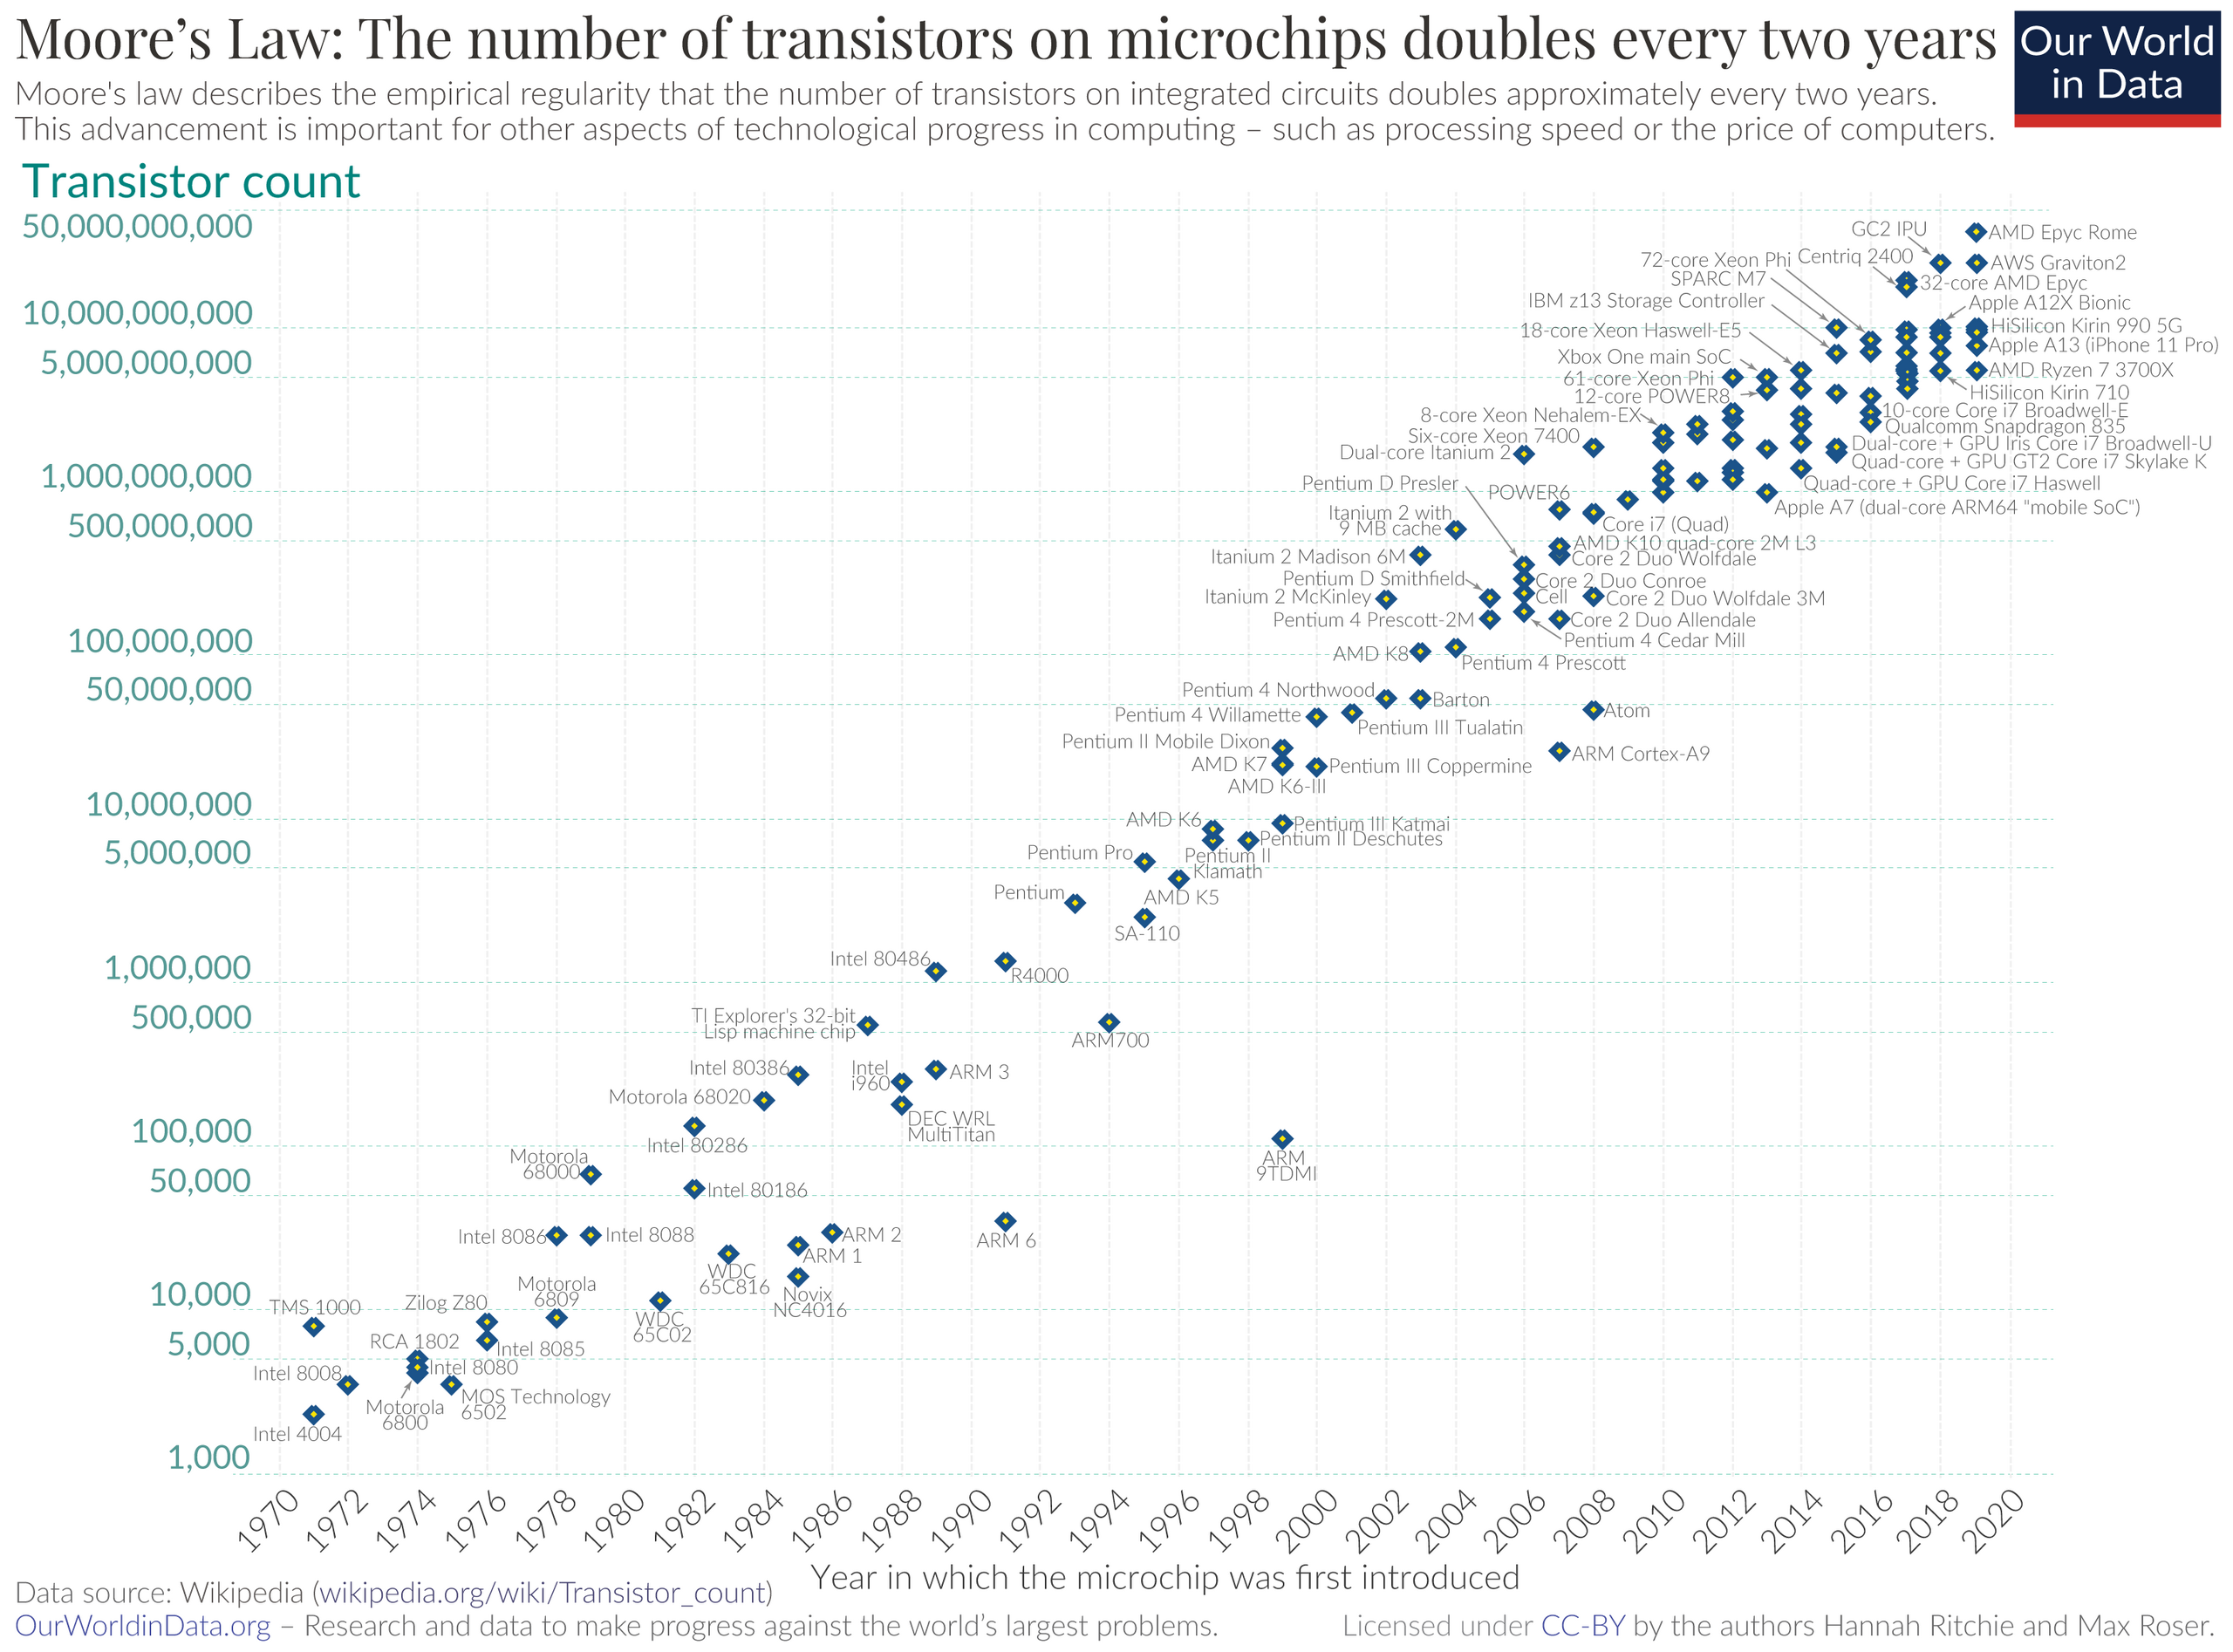
\includegraphics[width=0.6\linewidth]{images/moore.png}
%     \caption{Llei de Moore. Gràfic de quantitat de transistors MOS per any. Wikipedia.}
%     \label{<label>}
% \end{figure}

A continuació, repassarem la història del CMOS, analitzarem els principis físics i el seu funcionament intern, especialment orientat a l'electrònica digital, i explorarem les seves aplicacions actuals i futures, mostrant perquè continua sent una tecnologia essencial en el desenvolupament tecnològic modern.

\section{Història del CMOS}
% Destacar los hitos importantes desde 1963, comparaciones con tecnologías anteriores (nMOS, BJT).
% Mencionar su adopción masiva en los años 80-90 y cómo ha evolucionado.

\subsection{BJT i MOSFET}

\begin{wrapfigure}{r}{0.25\paperwidth}
    \centering
    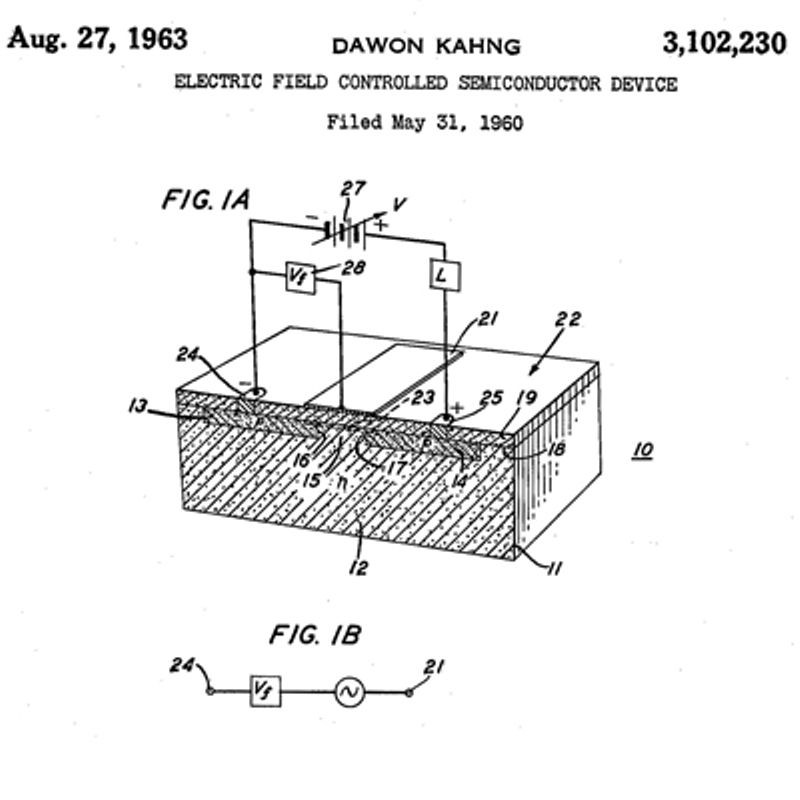
\includegraphics[width=\linewidth]{images/patent kahang.jpg}
    \caption{Patent \texttt{US3102230A} estatunidenca del MOSFET de Dawon Kahng.}
\end{wrapfigure}
Al final dels anys 1940, el transistor bipolar de junció, o BJT, va ser inventat per John Bardeen i Walter Brattain sota la direcció de William Shockley als laboratoris Bell Telephone. Gràcies a certes millores introduïdes de cara a l'eficiència, tant en el seu ús com a la seva producció, van ser introduïts al públic general als principis dels anys 1950 i van ser la tecnologia predominant al mercat durant trenta anys.


Prèviament, el transistor d'efecte de camp semiconductor-òxid-metall, o MOSFET, ja s'havia inventat i patentat a Europa. Aquest va ser objecte d'estudi per part de l'equip dels laboratoris Bell, però sense èxit, a causa dels problemes dels estats superficials \footnote{Els estats superficials són els estats electrònics que es formen a la superfície dels materials, deguts a la interrupció de la malla atòmica del material que acaba en la superfície. Aquest efecte es pot pal$\cdot$liar amb la \textit{passivització} de la superfície, que redueix l'efecte i estabilitza els estats electrònics al límit del material.} no va ser possible la seva adopció a gran escala.

Després d'avenços amb el transistor (òxid de Silici com a passivitzador, invenció de la tecnologia de fabricació planar), finalment Mohamed Atalla i Dawon Kahng van introduir el primer transistor MOS de silici funcional als laboratoris Bell l'any 1960. 

Tot i això, els transistors MOSFET no estaven a l'altura dels BJT de l'època i eren vistos com a inferiors. La principal diferència entre els MOSFET i BJT és el consum elèctric i el seu ús típic: 
\begin{itemize}
    \item Els BJT són controlats per corrent a la base, i aquest corrent controla el flux entre el col·lector i l'emissor. Tenen un comportament lineal i són ideals per a circuits analògics. Requereixen un flux de corrent constant per funcionar.
    \item Els MOSFET, quan s'utilitzen en configuració CMOS, només consumeixen energia durant els canvis d'estat (commutació), cosa que els fa especialment adequats per a circuits digitals. Fora de CMOS, els MOSFET pMOS i nMOS per separat també poden consumir energia de forma contínua segons com estiguin polaritzats.
\end{itemize}


El primer circuit integrat amb tecnologia MOSFET (únicament pMOS) va ser presentat al 1964 per General Microelectronics i el primer aparell d'us quotidià (una calculadora) amb aquests circuits va ser presentada per la mateixa empresa un any després\autocite{general_microelectronics}.
\begin{wrapfigure}{r}{0.2\paperwidth}
    \centering
    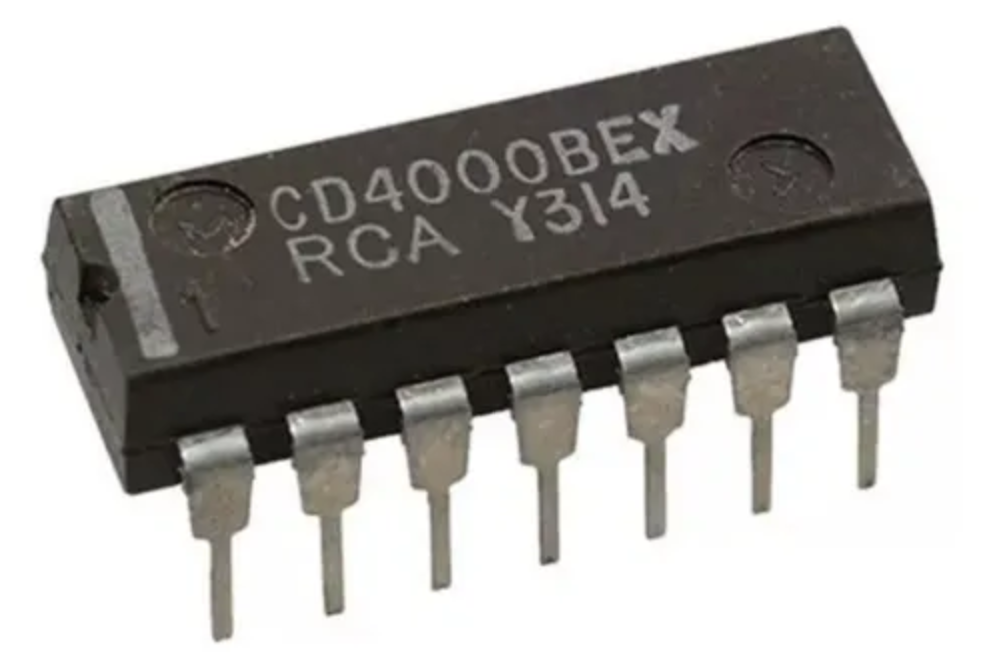
\includegraphics[width=\linewidth]{images/rca cd4000 chip.png}
    \caption{Xip de la família CD4000 de RCA.}
    \vspace{-1.3cm}
\end{wrapfigure}

\subsection{Naixement del CMOS, primers dispositius}

A mesura que augmentava la densitat dels circuits integrats, el consum energètic i la dissipació tèrmica eren limitacions greus. Això va motivar la recerca de tecnologies més eficients, i el CMOS va ser presentat com una solució prometedora el 1960 per la companyia Fairchild Semiconductor, tenint el seu primer contacte amb el públic el 1968 amb la presentació del xip lògic general CD4000 per RCA\autocite{wiki:4000-series_integrated_circuits}.

Del 1960 al 1980 va ser acceptat de forma àmplia, però van trobar problemes, entre ells un a causa de l'ús dels pMOS dins del CMOS, on els forats són els portadors i la seva mobilitat és inferior a la dels electrons ($\mu_e = \qty{1400}{\centi\meter\squared\per\volt\per\second} \gg \mu_h = \qty{450}{\centi\meter\squared\per\volt\per\second}$), fent reduir la velocitat d'operació del dispositiu. Aquesta limitació va fer sorgir altres alternatives com tecnologia Lògica d'Injecció Integrada, o I$^2$L i al principi dels anys 1980 hi havia una previsió de que CMOS seria desbancat pels mateixos dispositius I$^2$L. 

Però gràcies a la millora en la síntesi dels materials i litografia van poder fer integrar més dispositius CMOS en menys espai (complint així la Llei de Moore). També va arribar un punt on la fabricació de CMOS no era més difícil que la fabricació nMOS, fent així que es consolidés aquesta tecnologia.

\subsection{Actualitat}

Amb el pas del temps, aquesta tecnologia (en general els MOSFET) ha acabat sent una part fonamental de la vida de molta gent, en concret els CMOS ho han sigut a causa del seu baix consum i la seva alta densitat i facilitat de disseny i fabricació. 

Alguns dels dispositius més notables construïts amb aquesta tecnologia són:
\begin{itemize}
    \item Microprocessadors PowerPC de la família 600. En especial el xip PowerPC 620, sent dels primers en treballar en arquitectura de 64 bits.
    \item Microprocessadors Intel de la gamma 8000 i 80000, que utilitzen tecnologia CHMOS, culminant en l'arxiconegut processador Intel Pentium (que utilitza CMOS bipolars de $\qty{800}{\nano\meter}$).
    \item La consola Nintendo Wii, on el seu microprocessador \textit{Hollywood} està fabricat amb tecnologia CMOS de $\qty{90}{\nano\meter}$.
    \item Càmeres astronòmiques com la C-BLUE One i les Teledyne COSMOS.
\end{itemize}

\section{Funcionament intern}

El funcionament intern dels CMOS es basa en tot el funcionament darrere dels MOSFET de tipus P i N. La complementació dels dos funcionaments ens permet començar a operar funcions lògiques en un circuit digital.

\subsection{Formació del canal}

\begin{wrapfigure}{l}{0.25\paperwidth}
    \centering
    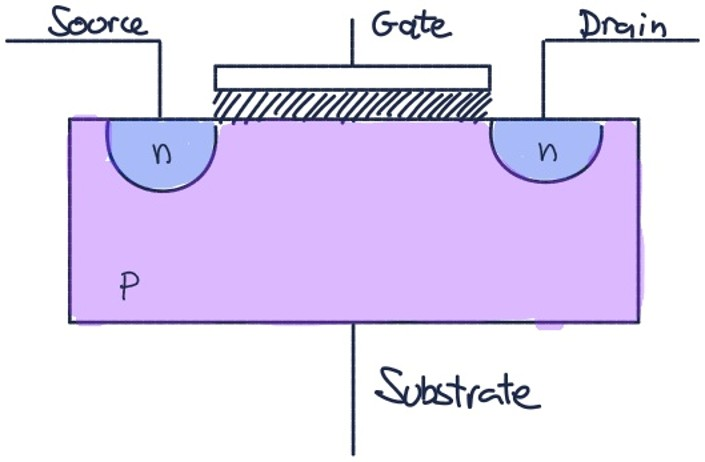
\includegraphics[width=\linewidth]{images/nmos1.jpg}
    \caption{Estructura d'un NMOS}
    \label{fig:nmos1}
    \vspace{-0.3cm}
\end{wrapfigure}
El fet diferenciador del CMOS no es pot explicar si no és amb el funcionament complementari dels p i n MOS. Mirarem únicament el nMOS, el pMOS tindrà un funcionament exactament igual, però complementari.


Un dispositiu nMOS (Figura \ref{fig:nmos1}) consta de 4 contactes: Font, Drenatge, Substrat i Porta. L'estructura del nMOS és de la concatenació de semiconductors NPN amb un òxid format sobre el semiconductor P (que seria el substrat) amb un metall a l'altra banda de l'òxid. Aquest òxid i metall amb el semiconductor és el que dona el nom de MOS. Com a tal, l'estructura de substrat-òxid-metall, actuarà com un condensador elèctric, amb una tensió de ruptura associada.

Estant en equilibri entre el D i S ($V_D - V_S = V_{DS} = \qty{0}{\volt}$) si apliquem un voltatge entre la porta i substrat positiu hi haurà un camp elèctric localitzat entre el Substrat i la Porta. Això farà que els electrons que venen des del contacte del substrat viatgin cap a la porta, però seran interromputs per l'òxid, que és aïllant. L'acumulació d'electrons a la interfície entre el substrat i l'òxid crearà un pont entre els semiconductors de Font i Drenatge.


\begin{figure}[h]
    \centering
    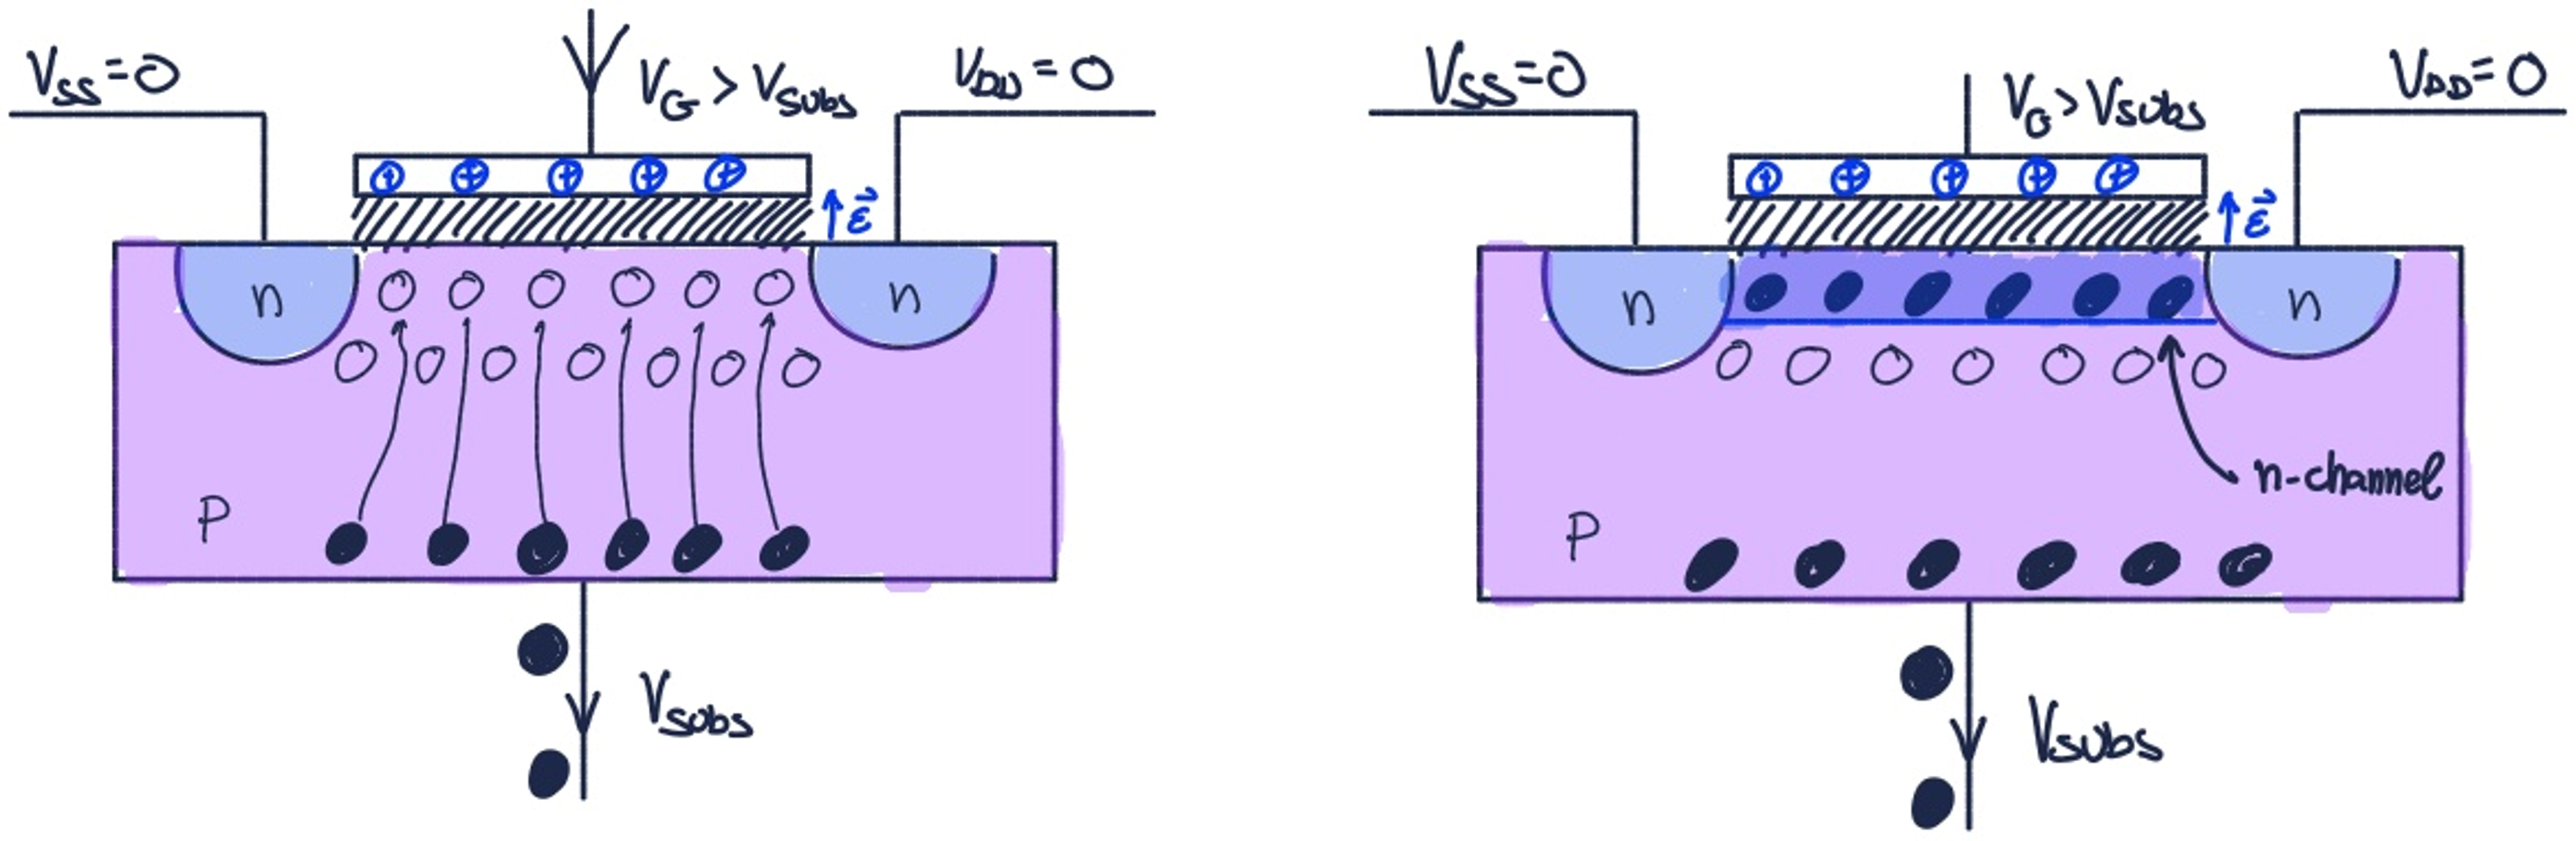
\includegraphics[width=0.6\paperwidth]{images/nmos23.png}
    \caption{Formació del canal en equilibri a $V_D$ = $V_S$}
    \label{fig:nmos23}
\end{figure}

Habitualment els dispositius MOSFET connecten el Substrat amb el Source. Ara bé, quan volem fer passar un volatge entre el source i el drain, el canal tindrà una amplada inversament proporcional a la distància recorreguda. Aquest fet farà que hagi una intensitat d'electrons variable en funció de la diferència de potencial, que serà la regió de tríode de la gràfica $I_D(V_{DS})$. 

Finalment si arribem a un voltatge de saturació $V_T$ la corrent serà estable i el canal estarà plenament format.

\begin{figure}[h]
    \centering
    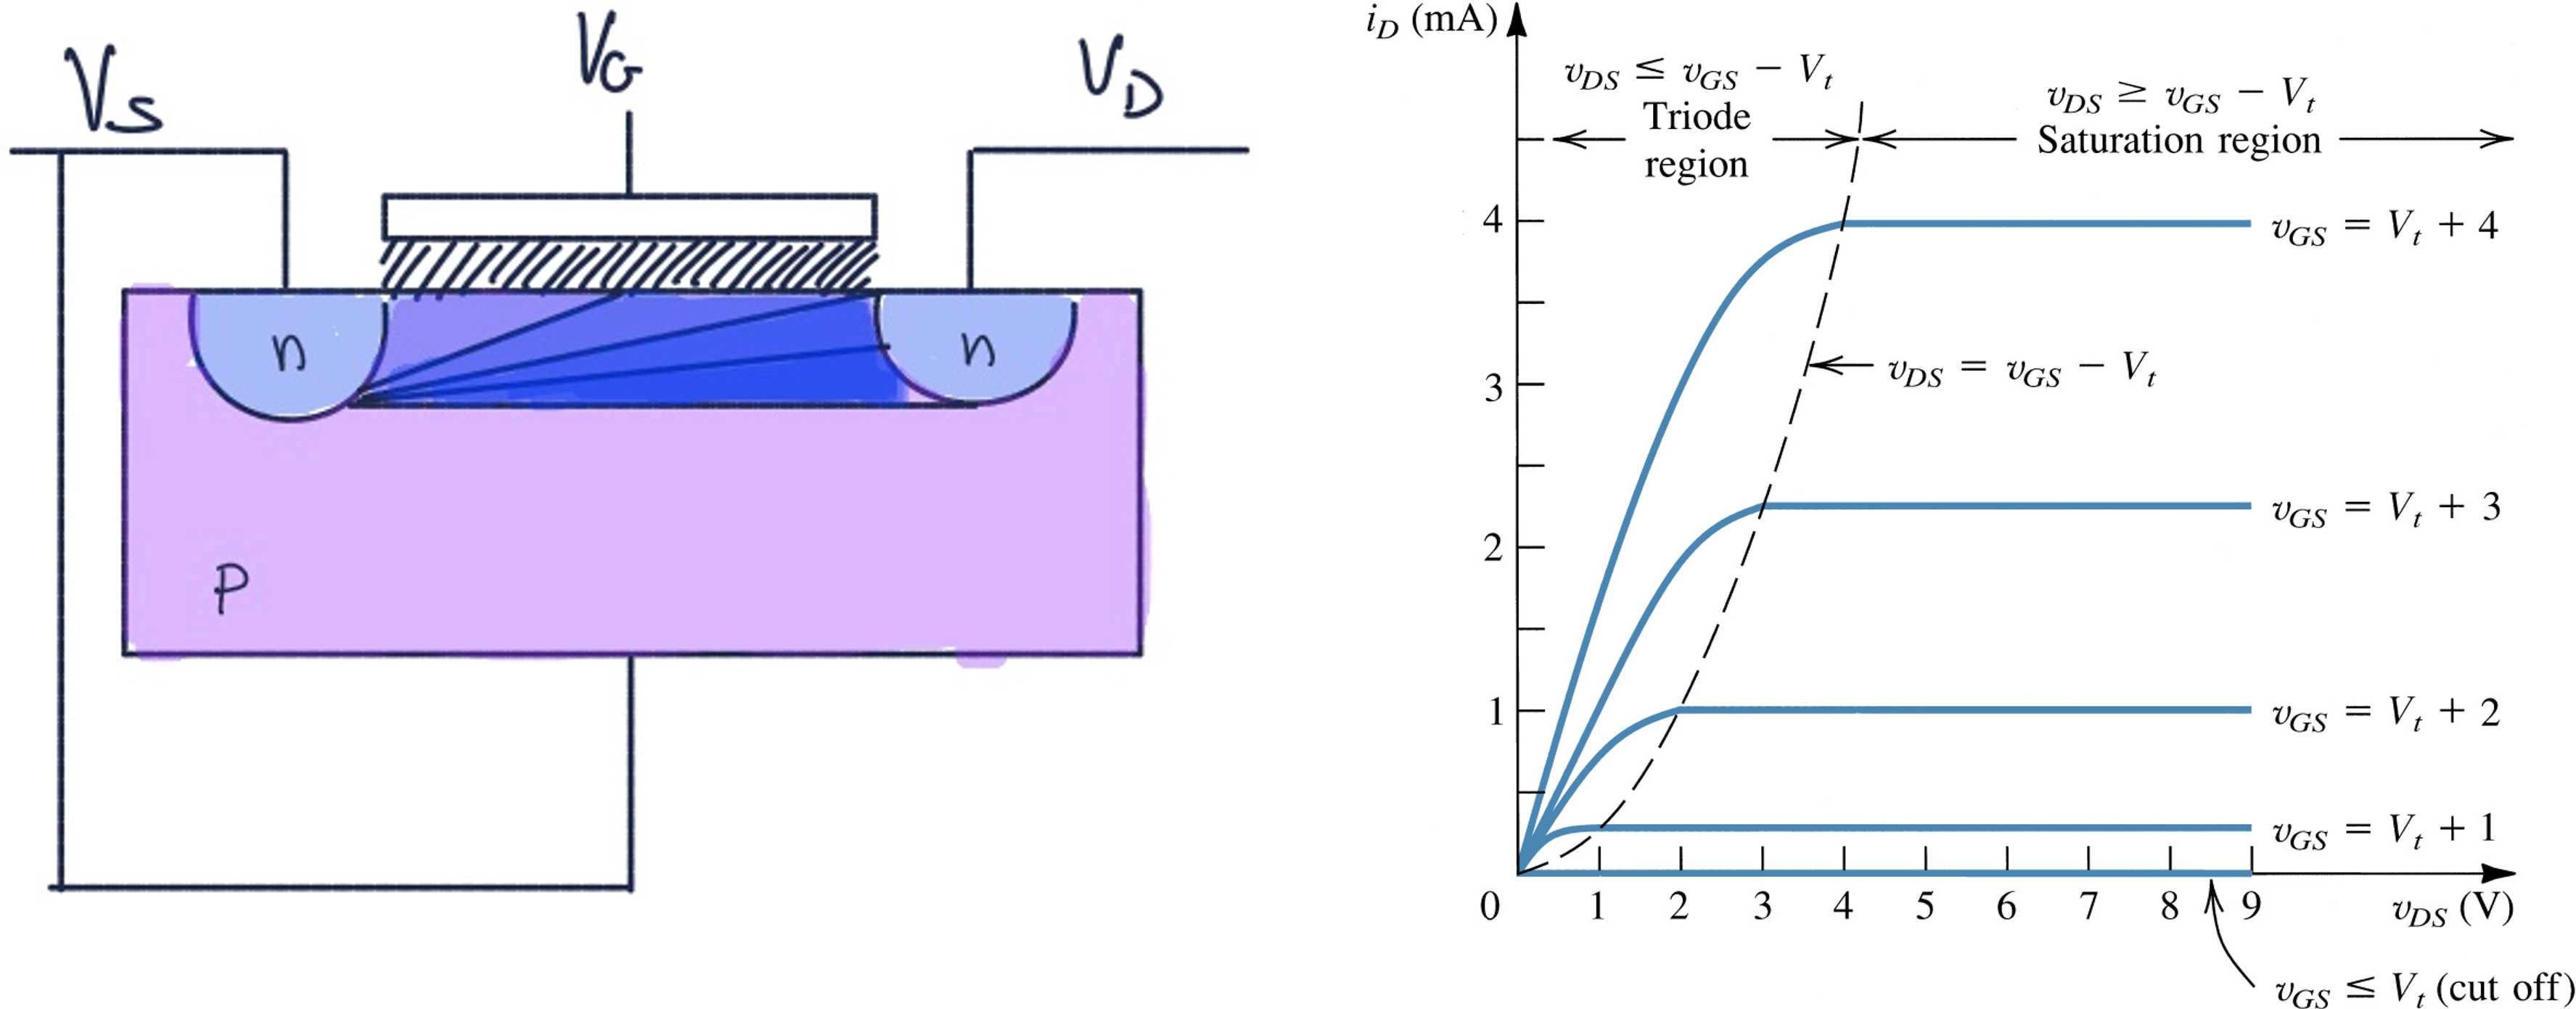
\includegraphics[width=0.6\paperwidth]{images/nmos idvds.png}
    \caption{A l'esquerra, els canals formats amb diferents regions: sense canal, punt de contacte, regió triódica i regió de saturació. A la dreta la gràfica $I_D(V_{DS})$ amb cada una de les regions.}
    \label{fig:nmos23}
\end{figure}

\subsection{Estructura d'un CMOS, senyals 0 i 1}


\subsection{Estructura d'un CMOS}

\begin{wrapfigure}{l}{0.2\paperwidth}
    \centering
    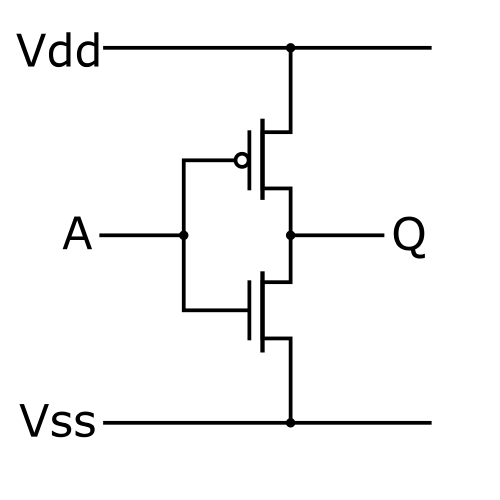
\includegraphics[width=\linewidth]{images/CMOS_inverter.png}
    \caption{Estructura d'un inversos CMOS}
    \vspace{-0.5cm}
\end{wrapfigure}


Lorem ipsum dolor sit amet, consectetur adipiscing elit. Nullam et sagittis nulla. Donec blandit volutpat venenatis. Maecenas sodales at libero nec tempus. Maecenas sit amet ullamcorper neque. Curabitur vitae imperdiet leo. Curabitur molestie nibh sed magna scelerisque gravida. Pellentesque in risus tortor.

Integer porta lectus nisi, non malesuada arcu imperdiet sed. Quisque ut justo tempor, lacinia eros pellentesque, faucibus urna. Etiam nisi eros, rutrum vitae neque id, posuere dignissim libero. Nunc ut neque fermentum, fermentum urna at, tincidunt nulla. Mauris in nulla dignissim, rutrum est ut, tempor nunc. Morbi dictum odio luctus tortor luctus, eu tincidunt enim placerat. Morbi tempor egestas feugiat. Donec imperdiet condimentum bibendum. Aliquam vitae tellus felis. Pellentesque imperdiet feugiat dictum. Pellentesque sodales turpis nec placerat tempor. Mauris tincidunt mauris ac rutrum interdum. Pellentesque sit amet aliquam tortor.

Nunc maximus nulla ut sapien ullamcorper pellentesque. In hac habitasse platea dictumst. Phasellus sed ligula aliquam, hendrerit ligula et, porttitor arcu. Vivamus ac lectus ut elit aliquet ornare a at justo. Vestibulum ornare, diam ornare congue blandit, risus dolor fringilla lorem, tincidunt viverra diam libero id augue. Mauris venenatis aliquet lorem ac tempus. Proin rutrum elementum nulla, sed lobortis turpis tristique non. Etiam ac odio maximus, hendrerit justo et, luctus enim. Phasellus volutpat dolor eu tortor tincidunt porta. In sed sapien vel sem placerat lacinia. Morbi mattis venenatis dictum. Nullam eleifend massa sit amet dui bibendum placerat.

Mauris velit enim, accumsan ac posuere consequat, malesuada in nisi. Duis euismod ac nisl quis rutrum. Duis consequat arcu eget erat aliquam suscipit. Vestibulum mollis ultricies urna, at viverra diam porta eu. Sed tristique justo semper, aliquam arcu sit amet, blandit nisl. Donec mollis molestie convallis. Nulla finibus lacus vitae dui porttitor mattis. Curabitur convallis felis vel sem mattis, quis dignissim lectus porttitor. Phasellus et risus quis lectus scelerisque gravida at eget odio. Ut vel mi quis turpis suscipit rutrum. Cras iaculis rutrum nulla, a elementum felis feugiat vel. Nulla at fringilla augue. Cras pulvinar, massa et ultricies aliquam, erat risus commodo magna, nec molestie turpis elit a erat.

Nam volutpat interdum neque ut eleifend. Aenean lobortis purus erat, in bibendum erat egestas ut. Pellentesque quis fringilla risus. Donec porta bibendum quam. Vivamus venenatis quam sit amet risus lacinia finibus. Curabitur placerat auctor ullamcorper. Aenean dictum, diam vel consectetur porta, enim erat tristique orci, eget vestibulum orci orci id risus. Cras egestas velit turpis. 
% Describir un inversor básico nMOS/pMOS en serie con explicación de entrada/salida.

\subsection{Bandes d'energia}
% Explicar las bandas de valencia/conducción en nMOS y pMOS, con comentario sobre inversión de canal.
% Comentar brevemente el modelo de portadores mayoritarios.


\section{Aplicacions}

\subsection{Portes lògiques}

\subsection{Sensors i cameres digitals}
% Cámaras digitales, sensores industriales, robótica.

\printbibliography

\end{document}
